\documentclass{article}
\usepackage{tikz}
\usepackage{amssymb}
\usepackage{amsmath}
\usepackage{geometry}
\geometry{margin=1.75cm}
\usetikzlibrary{shapes,arrows,positioning,calc,fit,backgrounds,shapes.geometric}


\begin{document}

% TGD - Big Picture
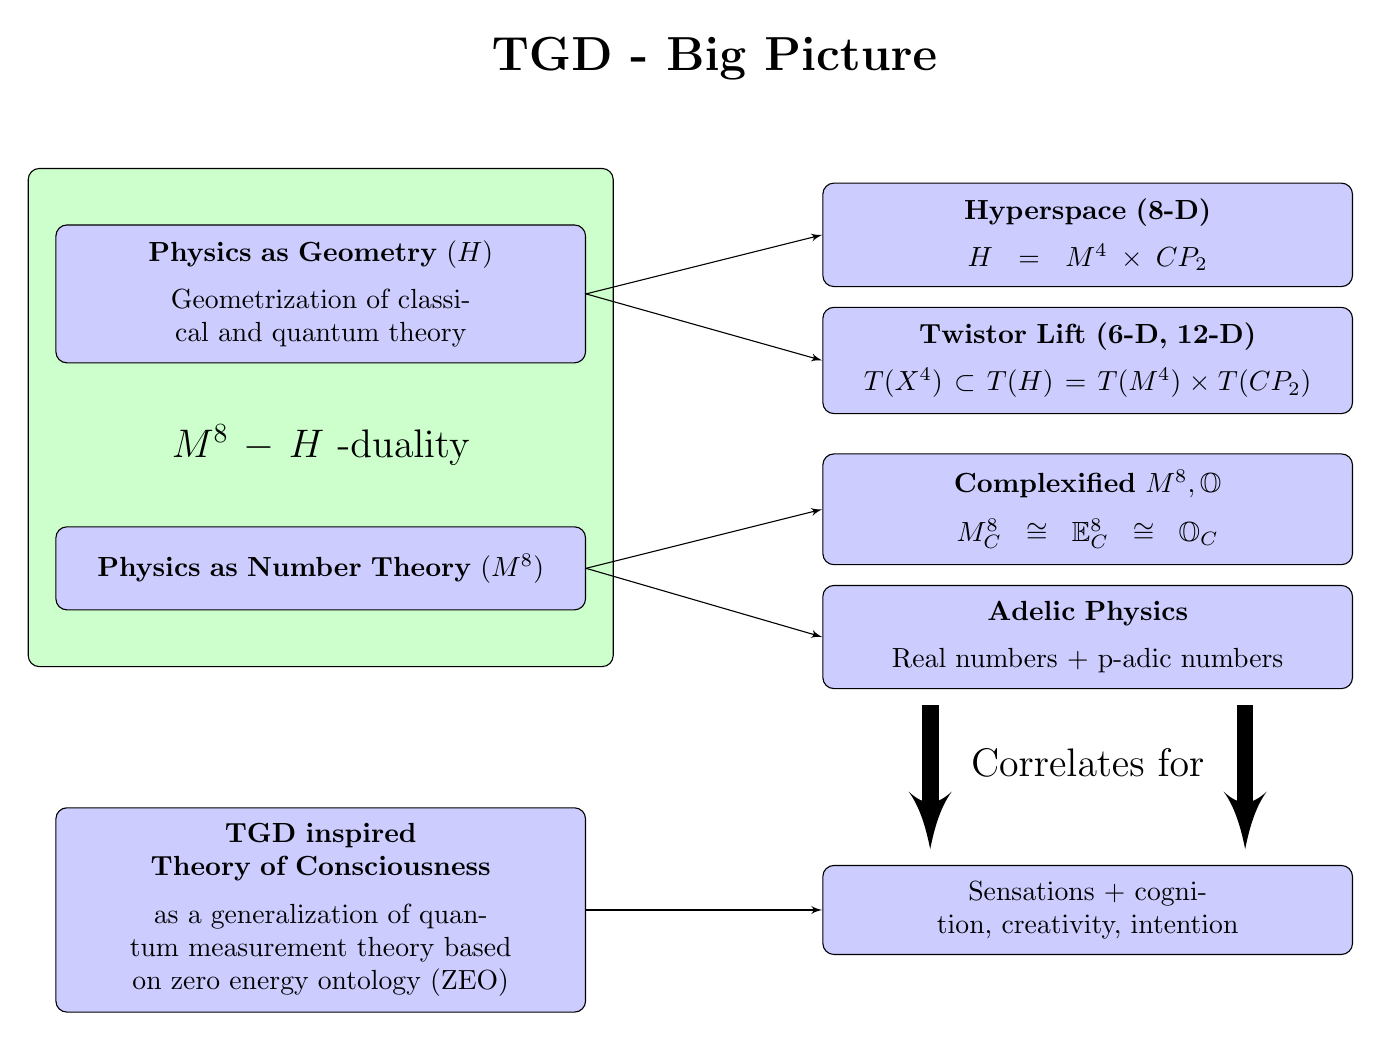
\begin{tikzpicture}[node distance=2cm]
\tikzstyle{block} = [rectangle, draw, fill=blue!20, text width=18em, text centered, rounded corners, minimum height=3em, inner sep=0.2cm]
\tikzstyle{line} = [draw, -latex']
\tikzstyle{thickarrow} = [draw, -latex', line width=6pt]

% Green Parent Box with adjusted placement
\node [block, draw, fill=green!20, minimum height=18em, text width=20em] (parentBox) {};

\node [above=1cm of parentBox, font=\LARGE\bfseries, xshift=5cm] (title) {TGD - Big Picture};

% Inside the Green Parent Box
\node [block] (physicsGeo) at ([yshift=-1.6cm]parentBox.north) {\textbf{Physics as Geometry $(H)$} \\[0.5em] Geometrization of classical and quantum theory};
\node [block, draw=none, fill=green!20, below=0.5cm of physicsGeo, font=\fontsize{14}{17}\selectfont] (duality) {$M^8-H$ -duality};
\node [block, below=0.5cm of duality] (physicsNumber) {\textbf{Physics as Number Theory $(M^8)$}};

% Other blocks
\node [block, right=3cm of physicsGeo, yshift=0.75cm] (hyperspace) {\textbf{Hyperspace (8-D)} \\[0.5em] $H = M^4 \times CP_2$};
\node [block, below=0.25cm of hyperspace] (twistor) {\textbf{Twistor Lift (6-D, 12-D)} \\[0.5em] $T(X^4) \subset T(H) = T(M^4) \times T(CP_2)$};
\node [block, right=3cm of physicsNumber, yshift=0.75cm] (complexM8) {\textbf{Complexified $M^8, \mathbb{O}$ \\[0.5em] $M^8_C \cong \mathbb{E}_C^8 \cong \mathbb{O}_C$}};
\node [block, below=0.25cm of complexM8] (adelicPhysics) {\textbf{Adelic Physics} \\[0.5em] Real numbers + p-adic numbers};

\node [block, below=2.5cm of physicsNumber] (consciousness) {\textbf{TGD inspired \\ Theory of Consciousness} \\[0.5em] as a generalization of quantum measurement theory based on zero energy ontology (ZEO)};

\node [block, draw=none, fill=white!20, below=0.4cm of adelicPhysics, font=\fontsize{14}{17}\selectfont] (analogy) {Correlates for};

\node [block, right=3cm of consciousness] (cognition) {Sensations + cognition, creativity, intention};

% Connections
\draw [line] (physicsGeo.east) -- (hyperspace.west);
\draw [line] (physicsGeo.east) -- (twistor.west);
\draw [line] (physicsNumber.east) -- (complexM8.west);
\draw [line] (physicsNumber.east) -- (adelicPhysics.west);
\draw [line] (consciousness.east) -- (cognition.west);

\draw [thickarrow] ($(adelicPhysics.south)-(2,0.2)$) -- ($(cognition.north)-(2,-0.2)$);
\draw [thickarrow] ($(adelicPhysics.south)-(-2,0.2)$) -- ($(cognition.north)-(-2,-0.2)$);

\end{tikzpicture}




\newpage % Page break for next diagram

% TGD - Induction
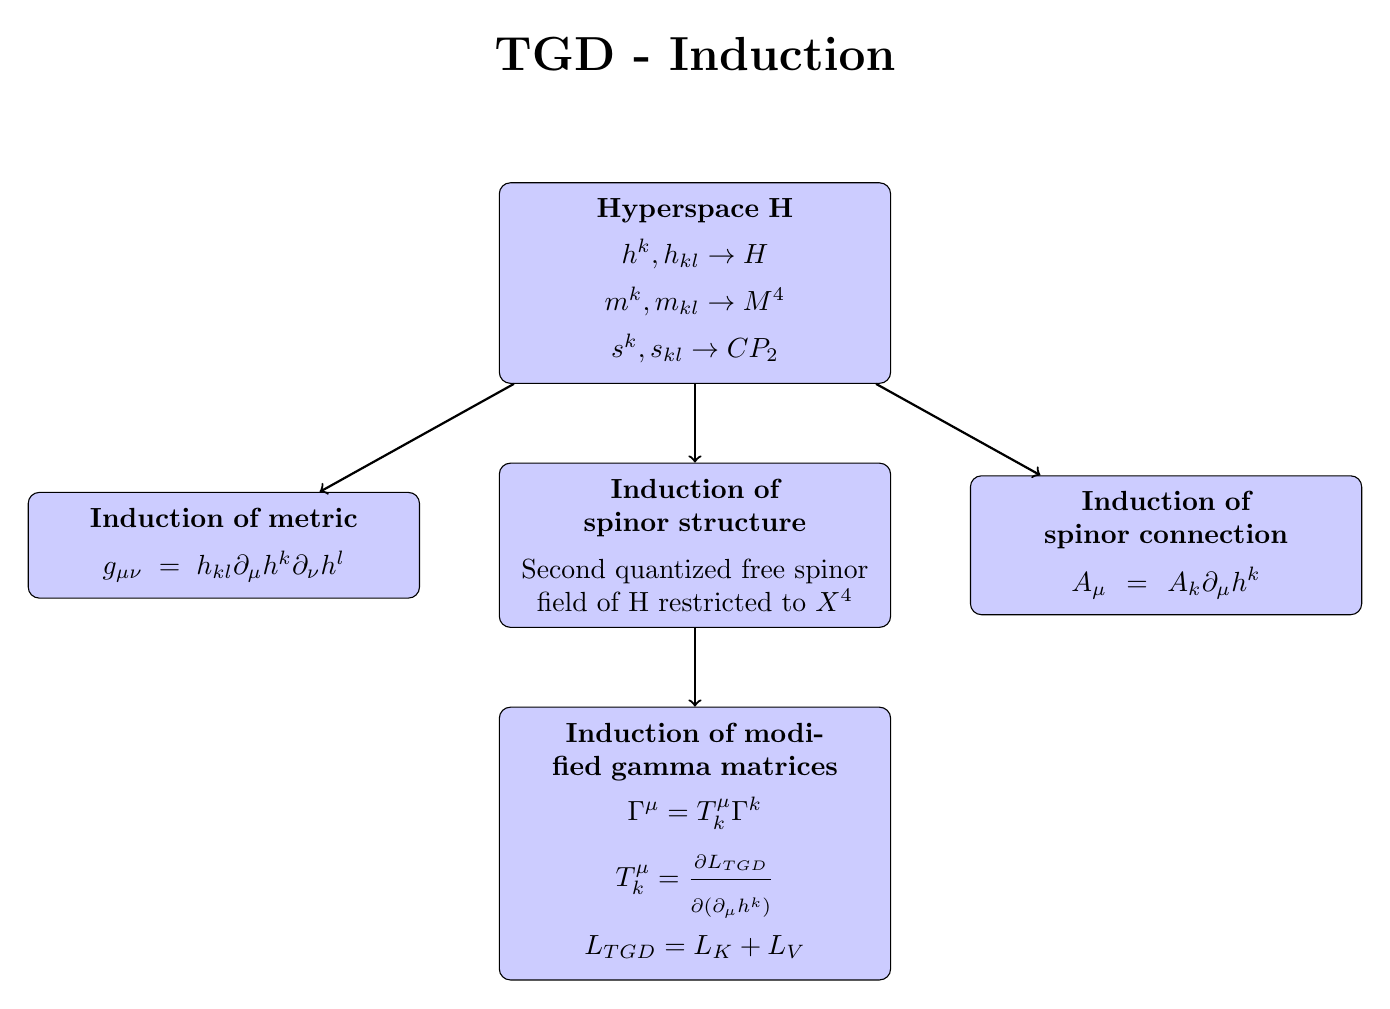
\begin{tikzpicture}[node distance=1cm]
\tikzstyle{block} = [rectangle, draw, fill=blue!20, text width=13em, text centered, rounded corners, minimum height=3em, inner sep=0.2cm]
\tikzstyle{line} = [draw, -latex']
\tikzstyle{thickarrow} = [draw, -latex', line width=6pt]

\node [font=\LARGE\bfseries, xshift=5cm] (title2) {TGD - Induction};

% Induction Blocks

\node [block, below=1.3cm of title2] (hyperspaceTransitions) {
    \textbf{Hyperspace H} \\[0.5em]
    \begin{tabular}{@{}c@{}}
        \( h^k, h_{kl} \rightarrow H \) \\[0.5em]
        \( m^k, m_{kl} \rightarrow M^4 \) \\[0.5em]
        \( s^k, s_{kl} \rightarrow CP_2 \)
    \end{tabular}
};

\node [block, below=1cm of hyperspaceTransitions] (spinorFieldInduction) {\textbf{Induction of spinor structure} \\[0.5em] Second quantized free spinor field of H restricted to \(X^4\)};

\node [block, left=1cm of spinorFieldInduction, yshift=0cm] (metricInduction) {\textbf{Induction of metric} \\[0.5em] \( g_{\mu\nu}= h_{kl}\partial_{\mu} h^k\partial_{\nu} h^l \)};

\node [block, right=1cm of spinorFieldInduction] (spinorConnectionInduction) {\textbf{Induction of spinor connection} \\[0.5em] \( A_{\mu}= A_k\partial_{\mu}h^k \)};

\node [block, below=of spinorFieldInduction] (gammaMatricesInduction) {
    \textbf{Induction of modified gamma matrices} \\[0.5em]
    \begin{tabular}{@{}c@{}}
        \( \Gamma^{\mu}=T^{\mu}_k\Gamma^k \) \\[0.5em]
        \( T^{\mu}_k = \frac{\partial \vphantom{\big(} L_{TGD}}{\partial \vphantom{\Big(} (\partial_{\mu} h^k)} \) \\[0.5em]
        \( L_{TGD} = L_K + L_V \)
    \end{tabular}
};

% Connections
\draw [->, thick] (hyperspaceTransitions) -- (metricInduction);
\draw [->, thick] (hyperspaceTransitions) -- (spinorFieldInduction);
\draw [->, thick] (hyperspaceTransitions) -- (spinorConnectionInduction);
\draw [->, thick] (spinorFieldInduction) -- (gammaMatricesInduction);

\end{tikzpicture}




\newpage % Page break for next diagram

% TGD - Group-wise
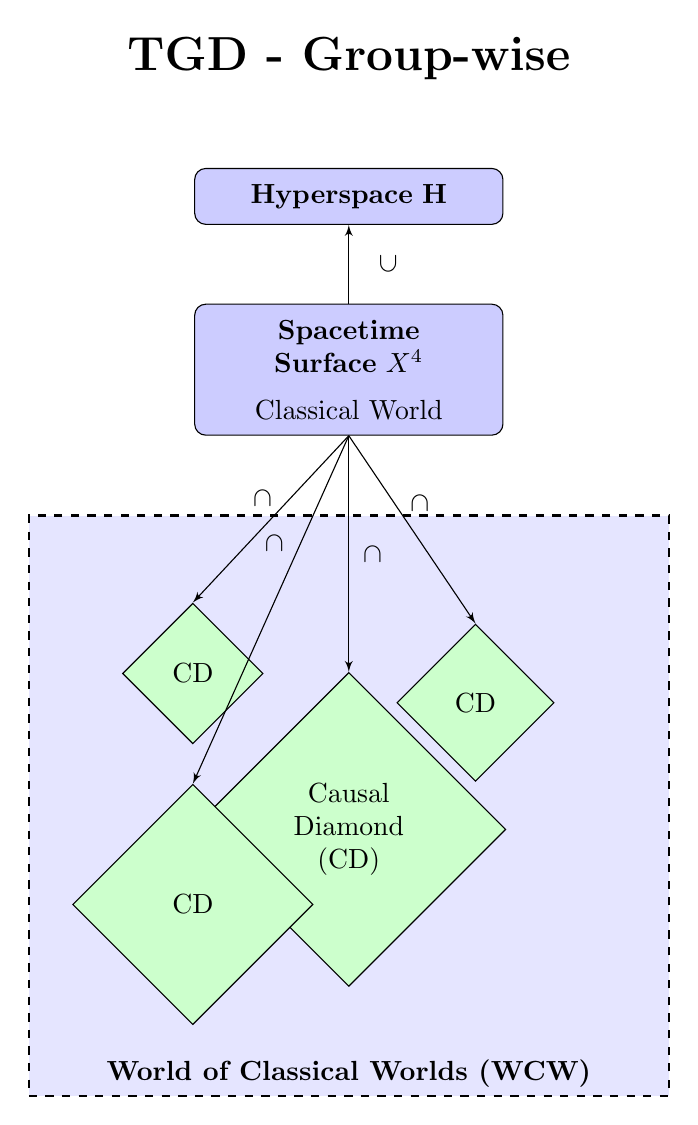
\begin{tikzpicture}[node distance=1cm]
\tikzstyle{block} = [rectangle, draw, fill=blue!20, text width=10em, text centered, rounded corners, minimum height=2em, inner sep=0.2cm]
\tikzstyle{diamondshape} = [diamond, draw, fill=green!20, text width=4em, align=center, inner sep=0.1cm]
\tikzstyle{subset} = [draw, -latex']
\tikzstyle{bigbox} = [rectangle, draw, thick, dashed, fill=blue!10, inner sep=1cm]


% Center the title at the top of the picture
\node [font=\LARGE\bfseries] (title) {TGD - Group-wise};

% Hyperspace H
\node [block, below=of title] (hyperspaceH) {\textbf{Hyperspace H}};

% Spacetime Surface X^4
\node [block, below=of hyperspaceH] (x4) {\textbf{Spacetime Surface} \(X^4\) \\[0.5em] Classical World};

\draw [subset] (x4) -- node[right=0.5cm, near start, rotate=90] {\(\subset\)} (hyperspaceH);

% CD diamonds (to be placed inside WCW later)
\node [diamondshape, below=3cm of x4, inner sep=1em] (cd1) {Causal Diamond (CD)};
\node [diamondshape, above left=0.75cm of cd1, inner sep=0.1em] (cd2) {CD};
\node [diamondshape, above right=0.15cm of cd1, inner sep=0.25em] (cd3) {CD};
\node [diamondshape, below=0.5cm of cd2, inner sep=1em] (cd4) {CD};

% WCW enclosing the CD nodes
\begin{pgfonlayer}{background}
\node[bigbox, fit=(cd1) (cd2) (cd3) (cd4), below=of x4] (wcw) {};
\node [anchor=south] at (wcw.south) {\textbf{World of Classical Worlds (WCW)}};
\end{pgfonlayer}

% Inclusion symbol from X^4 to one of the CDs
\draw [subset] (x4.south) -- node[right=0.3cm, yshift=-0.5cm, near start, rotate=-90] {\(\subset\)} (cd1.north);
\draw [subset] (x4.south) -- node[right=-0.6cm, near start, rotate=-90] {\(\subset\)} (cd2.north);
\draw [subset] (x4.south) -- node[right=0.5cm, near start, rotate=-90] {\(\subset\)} (cd3.north);
\draw [subset] (x4.south) -- node[right=-0.45cm, near start, rotate=-90] {\(\subset\)} (cd4.north);


\end{tikzpicture}



\newpage % Page break for next diagram

% TGD - Physical Interpretation
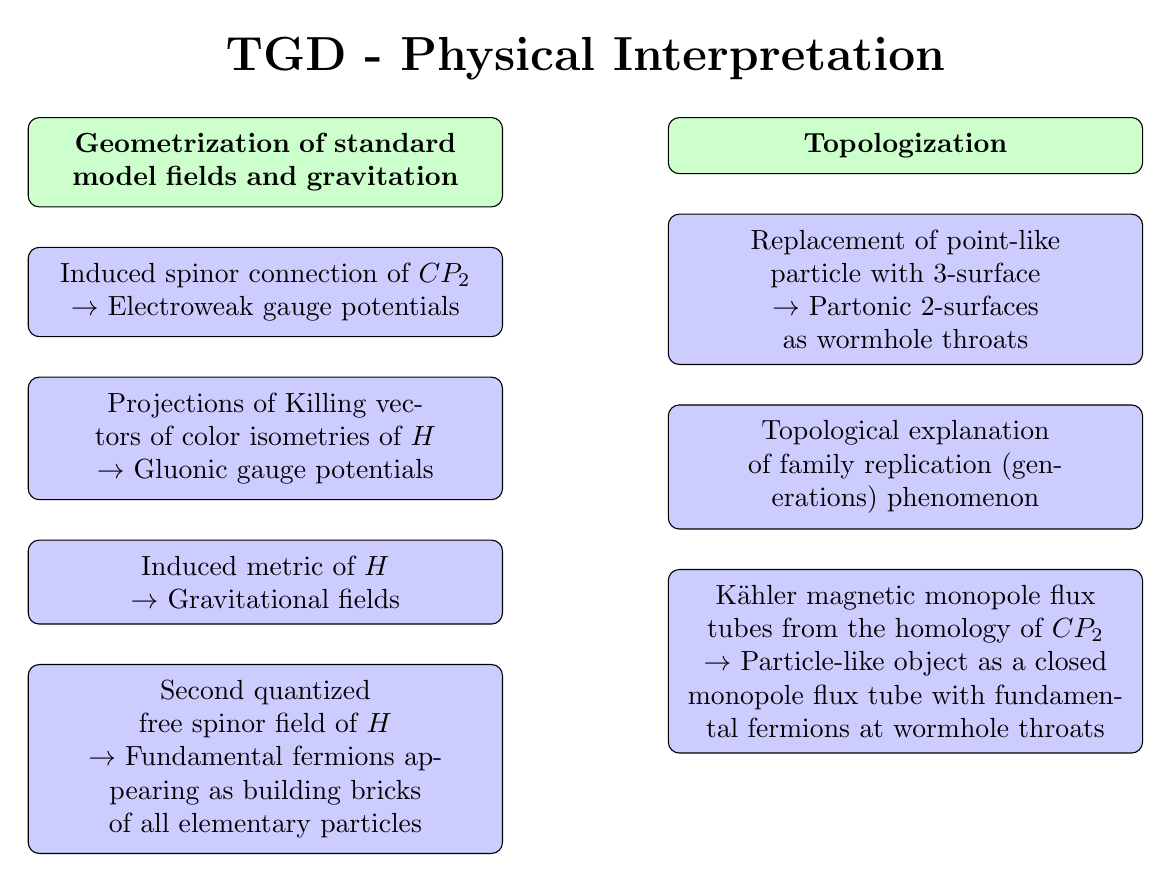
\begin{tikzpicture}[node distance=0.5cm]
\tikzstyle{block} = [rectangle, draw, fill=blue!20, text width=16em, text centered, rounded corners, minimum height=2em, inner sep=0.2cm]
\tikzstyle{greenblock} = [rectangle, draw, fill=green!20, text width=16em, text centered, rounded corners, minimum height=2em, inner sep=0.2cm]

% Center the title at the top of the picture
\node [font=\LARGE\bfseries] (title) {TGD - Physical Interpretation};

% Geometrization of standard model fields and gravitation
\node [greenblock, below left=of title, xshift=4cm ] (geomStandardModel) {\textbf{Geometrization of standard model fields and gravitation}};
\node [block, below=of geomStandardModel] (inducedSpinor) {Induced spinor connection of \(CP_2\) \\ \(\rightarrow\)  Electroweak gauge potentials};
\node [block, below=of inducedSpinor] (projectionsKilling) {Projections of Killing vectors of color isometries of \(H\) \\ \(\rightarrow\) Gluonic gauge potentials};
\node [block, below=of projectionsKilling] (inducedMetric) {Induced metric of \(H\)\\ \(\rightarrow\) Gravitational fields};
\node [block, below=of inducedMetric] (secondQuantized) {Second quantized free spinor field of \(H\)\\ \(\rightarrow\)  Fundamental fermions appearing as building bricks of all elementary particles };

% Topological aspects of TGD
\node [greenblock, below right=of title, xshift=-4cm] (topologicalAspects) {\textbf{Topologization}};
\node [block, below=of topologicalAspects] (replacementPoint) {Replacement of point-like particle with 3-surface\\ \(\rightarrow\) Partonic 2-surfaces
as wormhole throats};
\node [block, below=of replacementPoint] (topologicalExplanation) {Topological explanation of family replication (generations) phenomenon};
\node [block, below=of topologicalExplanation] (kahlerMagnetic) {Kähler magnetic monopole flux tubes from the homology of \(CP_2\)\\ \(\rightarrow\) Particle-like object as a closed monopole flux tube with fundamental fermions at wormhole throats};

\end{tikzpicture}


\end{document}
